% =============================================================================
% CSE 4224 — Progress / project report (pdfLaTeX, Overleaf-ready)
% =============================================================================
\documentclass[11pt,a4paper]{article}

\usepackage[margin=1in]{geometry}
\usepackage{booktabs}
\usepackage{hyperref}
\usepackage{enumitem}
\usepackage{parskip}
\usepackage{tikz}
\usetikzlibrary{arrows.meta,positioning,calc}

\hypersetup{colorlinks=true,linkcolor=blue!55!black,urlcolor=blue!55!black}

\setlist[itemize]{leftmargin=*}
\setlist[enumerate]{leftmargin=*}

\newcommand{\srcpath}{\texttt{DSD\_Project.srcs/sources\_1/new/}}
\newcommand{\simpath}{\texttt{DSD\_Project.srcs/sim\_1/new/}}
\newcommand{\conpath}{\texttt{DSD\_Project.srcs/constrs\_1/new/}}

\begin{document}

% -----------------------------------------------------------------------------
% 1. Front page
% -----------------------------------------------------------------------------
\begin{titlepage}
  \centering
  \vspace*{1.8cm}

  {\Large\bfseries CSE 4224}\\[0.35em]
  {\large Digital System Design Laboratory}

  \vspace{2.2cm}

  {\LARGE\bfseries Graph Explorer}\\[0.5em]
  {\Large BFS/DFS Hardware Path Search on Basys~3 (Verilog / Vivado)}

  \vfill

  \textbf{Implemented by}

  \vspace{1.1cm}

  \begin{minipage}{0.88\textwidth}
    \centering
    Name: \hrulefill \quad Student ID / Roll: \hrulefill

    \vspace{1.0cm}

    Name: \hrulefill \quad Student ID / Roll: \hrulefill
  \end{minipage}

  \vspace{1.8cm}

  \textbf{Date:} \hrulefill

  \vspace{2cm}
\end{titlepage}

\newpage
\setcounter{page}{1}

% -----------------------------------------------------------------------------
% 2. Project description
% -----------------------------------------------------------------------------
\section{Project description}

The \textbf{Graph Explorer} is a digital system that runs on the Digilent \textbf{Basys~3} board (Xilinx Artix-7). The user encodes a small directed graph (four nodes) on switches, selects a start node, a target node, a traversal mode (breadth-first or depth-first search), and whether to report \textbf{minimum} or \textbf{maximum} hop count along valid paths. The design then executes the chosen algorithm in hardware and shows the result on the seven-segment display, with LEDs and an RGB LED for status and visited feedback. The RTL is written in \textbf{Verilog} and organized as a top module, a core \texttt{graph\_engine}, memory for the graph and algorithmic structures, a central control finite-state machine, and peripheral blocks for debouncing, clock division, and display.

% -----------------------------------------------------------------------------
% 3. Project structure
% -----------------------------------------------------------------------------
\section{Project structure}

The design follows a clear hierarchy from simulation to silicon-oriented top level:

\begin{enumerate}
  \item \textbf{Testbench} (\texttt{tb\_graph\_explorer}) instantiates the hardware top and drives clocks, switches, and the center button for simulation.
  \item \textbf{Top RTL} (\texttt{graph\_explorer\_top}) connects board pins to internal logic: debounced button input, divided tick for multiplexed displays, the \texttt{graph\_engine} datapath, and seven-segment / RGB outputs.
  \item \textbf{Graph engine} (\texttt{graph\_engine}) wires together the \texttt{register\_set} (latched configuration), \texttt{memory\_unit} (adjacency, queue, stack), \texttt{control\_unit} (load sequence and BFS/DFS execution), and \texttt{graph\_alu} (simple combinational support).
\end{enumerate}

Data generally flows from switches and button events into the registers and control unit; the control unit reads and writes \texttt{memory\_unit} (edges, BFS queue, DFS stack) and updates display and LED outputs through the top-level glue.

\subsection{Flow diagram}

Figure~\ref{fig:flow} shows how signals move through \texttt{graph\_explorer\_top}: the button path is conditioned before entering \texttt{graph\_engine}; switches go directly to the engine; a divided tick runs the seven-segment multiplexer; and engine outputs drive LEDs, digits, and RGB (via \texttt{rgb\_status}). Inside the engine, the control unit orchestrates the register file, memory, and ALU slice.

\begin{figure}[htbp]
\centering
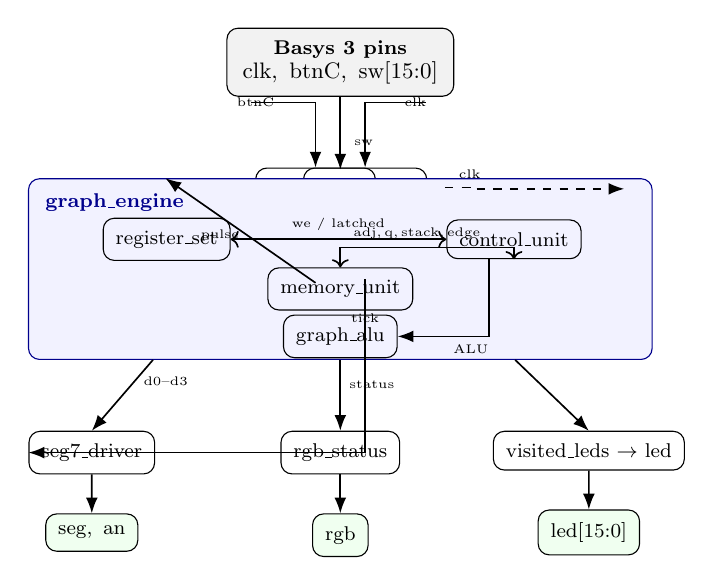
\begin{tikzpicture}[
  scale=0.9,
  transform shape,
  arr/.style={-{Latex},semithick},
  lbl/.style={font=\scriptsize, inner sep=1pt, fill=white, draw=none},
  blk/.style={draw, rounded corners, align=center, font=\footnotesize, inner sep=5pt},
  small/.style={font=\scriptsize}
]
  \node[blk, fill=gray!10, minimum width=3.2cm] (in)
    {\textbf{Basys~3 pins}\\\small clk,\, btnC,\, sw[15:0]};

  \node[blk, below left=1.0cm and 0.35cm of in.south, anchor=north] (deb) {debouncer};
  \node[blk, below=0.45cm of deb] (ed) {edge\_detector};
  \node[blk, below right=1.0cm and 0.35cm of in.south, anchor=north] (div) {clk\_divider};
  \node[blk, below=0.45cm of div] (tick) {tick $\approx$1\,kHz};

  \node[blk, below=1.15cm of in.south, minimum width=8.8cm, minimum height=2.55cm,
       fill=blue!5, draw=blue!55!black] (eng) {};
  \node[anchor=north west, font=\footnotesize\bfseries, text=blue!55!black] at ($(eng.north west)+(0.12,-0.1)$)
    {graph\_engine};

  % Top row: register file and control (memory below so arrows do not cross the wrong block)
  \node[blk] (reg) at ($(eng.center)+(-2.45,0.42)$) {register\_set};
  \node[blk] (cu) at ($(eng.center)+(2.45,0.42)$) {control\_unit};
  \node[blk] (mem) at ($(eng.center)+(0,-0.28)$) {memory\_unit};
  \node[blk] (alu) at ($(eng.center)+(0,-0.95)$) {graph\_alu};

  \draw[arr, <->] (reg.east) -- node[above, font=\tiny] {we / latched} (cu.west);
  \draw[arr, <->] (mem.north) -- ++(0,0.28) -| node[above, pos=0.22, font=\tiny] {adj,\,q,\,stack,\,edge} (cu.south);
  \draw[arr] (cu.south) ++(-0.35,0) |- node[pos=0.6, below, font=\tiny] {ALU} (alu.east);

  \node[blk, below=1.0cm of eng.south west, anchor=north, xshift=0.9cm] (seg)
    {seg7\_driver};
  \node[blk, below=1.0cm of eng.south, anchor=north] (rgbm) {rgb\_status};
  \node[blk, below=1.0cm of eng.south east, anchor=north, xshift=-0.9cm] (ledb)
    {visited\_leds $\rightarrow$ led};

  \node[blk, below=0.55cm of seg, fill=green!6] (out7) {seg,\, an};
  \node[blk, below=0.55cm of rgbm, fill=green!6] (outr) {rgb};
  \node[blk, below=0.55cm of ledb, fill=green!6] (outl) {led[15:0]};

  % Top-level inputs into engine
  \draw[arr] (in.south west) ++(0.35,-0.08) -| node[near start, left, font=\tiny] {btnC} (deb.north);
  \draw[arr] (in.south) -- node[right, font=\tiny, xshift=2pt, yshift=-4pt] {sw} ($(eng.north)+(0,0.12)$);
  \draw[arr] (ed.south) -- node[left, font=\tiny, pos=0.45] {pulse} ($(eng.north west)!0.22!(eng.north east)$);
  \draw[arr] (in.south east) ++(-0.4,-0.08) -| node[near start, right, font=\tiny] {clk} (div.north);

  \draw[arr] (tick.south) |- node[pos=0.15, above, font=\tiny] {tick} (seg.west);

  \draw[arr] ($(eng.south west)!0.2!(eng.south east)$) -- node[right, font=\tiny, pos=0.3] {d0--d3} (seg.north);
  \draw[arr] (eng.south) -- node[right, font=\tiny, pos=0.35] {status} (rgbm.north);
  \draw[arr] ($(eng.south west)!0.78!(eng.south east)$) -- (ledb.north);

  \draw[arr] (seg) -- (out7);
  \draw[arr] (rgbm) -- (outr);
  \draw[arr] (ledb) -- (outl);

  % clk to engine (simplified: horizontal from div area)
  \draw[arr, dashed] (div.east) ++(0.25,0) -- ++(0.35,0) |- node[pos=0.2, above, font=\tiny] {clk} ($(eng.north east)+(-0.4,-0.15)$);
\end{tikzpicture}
\caption{Data and control flow in \texttt{graph\_explorer\_top}: button conditioning, switch and clock distribution, internals of \texttt{graph\_engine}, and outputs to display and LEDs.}
\label{fig:flow}
\end{figure}

% -----------------------------------------------------------------------------
% 4. Project units with descriptions and implementation files
% -----------------------------------------------------------------------------
\section{Project units}

All RTL lives under \srcpath{} unless noted. The subsections below \textbf{describe every unit} in the project. Section~\ref{sec:memcu} then gives a \textbf{slightly longer} focus on the two largest behavioral blocks (\texttt{memory\_unit.v}, \texttt{control\_unit.v}). No source code is pasted here—only file names.

\subsection{Summary table}

\begin{table}[htbp]
  \centering
  \caption{Design units and implementation files.}
  \label{tab:units}
  \begin{tabular}{@{}p{0.26\textwidth}p{0.44\textwidth}p{0.24\textwidth}@{}}
    \toprule
    \textbf{Unit / module} & \textbf{Role} & \textbf{File(s)} \\
    \midrule
    \texttt{graph\_explorer\_top} &
    Top-level integration: I/O, debounce chain, clock divider, engine, segment and RGB drivers. &
    \texttt{graph\_explorer\_top.v} \\
    \addlinespace
    \texttt{debouncer} &
    Suppresses switch bounce on the center button before edge detection. &
    \texttt{debouncer.v} \\
    \addlinespace
    \texttt{edge\_detector} &
    Produces a one-cycle pulse from a stable button level. &
    \texttt{edge\_detector.v} \\
    \addlinespace
    \texttt{clk\_divider} &
    Generates a low-frequency tick for time-multiplexed seven-segment scanning. &
    \texttt{clk\_divider.v} \\
    \addlinespace
    \texttt{graph\_engine} &
    Structural wrapper connecting registers, memory, control, and ALU. &
    \texttt{graph\_engine.v} \\
    \addlinespace
    \texttt{register\_set} &
    Holds latched graph word, start/target indices, BFS/DFS flag, and min/max mode. &
    \texttt{register\_set.v} \\
    \addlinespace
    \texttt{memory\_unit} &
    Stores $4\times4$ adjacency, BFS FIFO, and DFS stack; services edge queries. &
    \texttt{memory\_unit.v} \\
    \addlinespace
    \texttt{control\_unit} &
    Main FSM: multi-step configuration, BFS shortest-hop search, DFS path enumeration for min/max length. &
    \texttt{control\_unit.v} \\
    \addlinespace
    \texttt{graph\_alu} &
    Small combinational block (documentation-oriented ALU slice). &
    \texttt{graph\_alu.v} \\
    \addlinespace
    \texttt{seg7\_driver} &
    Active-low segment patterns and anode multiplexing for four digits. &
    \texttt{seg7\_driver.v} \\
    \addlinespace
    \texttt{rgb\_status} &
    Maps a 2-bit status code to RGB LED drive. &
    \texttt{rgb\_status.v} \\
    \addlinespace
    Shared definitions &
    Optional parameters / constants for the graph core. &
    \texttt{graph\_defs.vh} \\
    \addlinespace
    Testbench &
    Simulation harness for the top module. &
    \texttt{tb\_graph\_explorer.v} \\
    \addlinespace
    Constraints &
    Basys~3 pin and timing constraints for implementation. &
    \texttt{basys3\_pins.xdc} \\
    \bottomrule
  \end{tabular}
\end{table}

\noindent\textbf{Locations:} RTL and \texttt{.vh} under \srcpath{}; testbench under \simpath{}; constraints under \conpath{}.

\subsection{Descriptions of all units}

\paragraph{\texttt{graph\_explorer\_top} (\texttt{graph\_explorer\_top.v}).}
This is the synthesizable top: it maps board pins (switches, center button, LEDs, seven-segment anodes/cathodes, RGB) to internal wires, instantiates the debouncer and edge detector for the button, the clock divider tick, the \texttt{graph\_engine}, and the display/status drivers. It is the module targeted for Basys~3 bitstream generation.

\paragraph{\texttt{debouncer} (\texttt{debouncer.v}).}
Filters mechanical bounce on the center button by requiring a stable raw level for many clock cycles before updating a debounced output. That clean level is what downstream logic treats as the ``real'' button state.

\paragraph{\texttt{edge\_detector} (\texttt{edge\_detector.v}).}
Watches the debounced button and emits a \textbf{single-cycle pulse} when a press edge is detected. The control unit uses that pulse as ``user confirmed this step'' without counting multiple transitions per physical press.

\paragraph{\texttt{clk\_divider} (\texttt{clk\_divider.v}).}
Divides the board clock to produce a slow \textbf{tick} used to time-multiplex the four seven-segment digits so only one anode is active at a time while the eye integrates a stable image.

\paragraph{\texttt{graph\_engine} (\texttt{graph\_engine.v}).}
A \textbf{structural} (non-behavioral) wrapper: it declares the interconnection between \texttt{register\_set}, \texttt{memory\_unit}, \texttt{control\_unit}, and \texttt{graph\_alu}, matching the datapath-plus-controller partition used in the lab report.

\paragraph{\texttt{register\_set} (\texttt{register\_set.v}).}
Holds configuration loaded from switches across the stepped workflow: the 16-bit adjacency word, start and target node indices, a flag for BFS versus DFS, and a flag for minimum versus maximum hop objective. Write enables come from the control unit on each configuration phase.

\paragraph{\texttt{memory\_unit} (\texttt{memory\_unit.v}).}
Central storage for the graph and algorithmic working data: the adjacency bit vector, a FIFO for BFS frontier nodes, and a stack for the iterative DFS path enumerator, plus combinational edge readout for indices $(i,j)$. (See Section~\ref{sec:memcu} for a concise summary of how it supports BFS/DFS.)

\paragraph{\texttt{control\_unit} (\texttt{control\_unit.v}).}
The main \textbf{finite-state machine}: multi-phase loading from switches, then either BFS distance search or DFS-based enumeration for min/max path length, while driving the memory ports and updating displays and status. (Section~\ref{sec:memcu} highlights the same file in more detail.)

\paragraph{\texttt{graph\_alu} (\texttt{graph\_alu.v}).}
A small \textbf{combinational} block (increment/compare style) kept as a separate module so the course block diagram explicitly includes an ``ALU'' slice next to the register file, even though much arithmetic also appears inside the control FSM.

\paragraph{\texttt{seg7\_driver} (\texttt{seg7\_driver.v}).}
Translates four BCD or hex nibbles from the control path into active-low segment patterns and sequences the anodes using the slow tick so four digits share one cathode bus.

\paragraph{\texttt{rgb\_status} (\texttt{rgb\_status.v}).}
Decodes a 2-bit status from the control unit into on/off patterns for the board’s red, green, and blue LEDs to show idle, busy, success, or error-style states at a glance.

\paragraph{Shared definitions (\texttt{graph\_defs.vh}).}
Optional Verilog header for shared parameters or constants (graph size, widths) so multiple \texttt{.v} files can stay consistent if constants are centralized.

\paragraph{Testbench (\texttt{tb\_graph\_explorer.v}).}
Simulation-only Verilog under \simpath{}: generates the clock, applies switch and button stimulus (often via tasks), and instantiates \texttt{graph\_explorer\_top} so behavior can be verified in the simulator without hardware.

\paragraph{Constraints (\texttt{basys3\_pins.xdc}).}
Xilinx constraints file under \conpath{}: maps logical ports to Basys~3 package pins and supplies basic timing constraints for implementation.

% -----------------------------------------------------------------------------
% 5. Brief description: memory unit and control unit (and their \texttt{.v} files)
% -----------------------------------------------------------------------------
\section{Brief description of the memory unit and control unit}
\label{sec:memcu}

These two modules contain most of the \textbf{algorithmic} RTL. Both are plain Verilog sources (no separate behavioral models).

\subsection{Memory unit — \texttt{memory\_unit.v}}
\textbf{Source file:} \texttt{memory\_unit.v} (\srcpath).

The memory unit stores the \textbf{directed} $4\times4$ adjacency as sixteen bits and answers \textbf{edge queries} used while expanding neighbors. For BFS it provides a \textbf{circular queue} (push, pop, empty, full) of node IDs. For DFS-style search over \textbf{simple paths} it provides a \textbf{stack} of packed records (node, neighbor index $k$, visited bitmask, depth). The \textbf{st\_poke} interface updates the top entry without popping so a parent frame can increment $k$ after trying a child—essential for iterative DFS in hardware. \textbf{clr\_qs} clears queue and stack for a new run while \textbf{adj\_we} reloads the graph from the register file when the user commits the switch pattern.

\subsection{Control unit — \texttt{control\_unit.v}}
\textbf{Source file:} \texttt{control\_unit.v} (\srcpath).

The control unit implements the \textbf{user protocol}: after reset, successive button pulses latch graph, start, target, and mode (BFS/DFS and min/max) into \texttt{register\_set} and into \texttt{memory\_unit} for the adjacency. It then enters \textbf{run} substates: for BFS, clear/init, enqueue start, dequeue/expand/test-target/enqueue neighbors with distance bookkeeping; for DFS, clear stack, push a start frame, then loop with stack peek, target test, neighbor advance (\textbf{poke} + optional child \textbf{push}), and pop when all neighbors are tried. It drives \texttt{memory\_unit.v} ports (\texttt{q\_*}, \texttt{st\_*}, \texttt{edge\_i}/\texttt{edge\_j}, \texttt{adj\_we}, \texttt{clr\_qs}) and updates \textbf{seven-segment} digits and \textbf{RGB} status for each phase and final outcome.

% -----------------------------------------------------------------------------
% 6. Discussion
% -----------------------------------------------------------------------------
\section{Discussion}

Partitioning the design into \texttt{memory\_unit} and \texttt{control\_unit} keeps \textbf{storage and connectivity} separate from the \textbf{long FSM} that implements both setup and two different graph algorithms. That split matches common practice in course-style datapath plus controller architectures and makes simulation easier: memory behavior (FIFO/stack) can be reasoned about independently of high-level BFS/DFS flow.

The Basys~3 offers limited human input (switches and one useful button), which led to a \textbf{stepped configuration workflow} rather than a full keyboard or UART interface. Representing a $4\times4$ adjacency on sixteen switches is workable for a lab demo but bounds graph size; the same architecture can be extended later with more storage and a wider control loop.

\textbf{Simulation} with \texttt{tb\_graph\_explorer.v} validates clocking and basic interaction without hardware. \textbf{Synthesis and on-board} testing remain important next steps to confirm timing, pin mapping (\texttt{basys3\_pins.xdc}), and real switch/button behavior against the ideal model.

% -----------------------------------------------------------------------------
% 7. Future work
% -----------------------------------------------------------------------------
\section{Future work}

\begin{itemize}
  \item Run full \textbf{Vivado implementation} (synthesis, place-and-route), close timing at the chosen clock, and record \textbf{LUT/FF/BRAM} usage for the final report.
  \item Exercise the design on \textbf{physical hardware}, tune debounce intervals if needed, and capture a short \textbf{demo checklist} (graph patterns, expected displays).
  \item Extend the testbench with \textbf{self-checking} cases (e.g., disconnected graph, single-edge path, start equals target) and longer runs to observe end-to-end waveforms.
  \item Explore \textbf{larger $N$} or multi-cycle graph loading (e.g., UART or multi-button flow) if course scope allows.
  \item Optional \textbf{UX} improvements: clearer seven-segment legends, single-step debug, or a written appendix formalizing BFS distance versus DFS simple-path enumeration.
\end{itemize}

\end{document}
